% Setup
\documentclass[a4 paper, 12pt]{article}

% Title
\title{COSC3000 - REPORT \\ Visualisation}
\author{Teanlouise}
\date{\today}

% Margins
\usepackage{geometry}
\geometry{margin=2cm}

% Images
\usepackage{graphicx}
\usepackage{float}
\usepackage[export]{adjustbox}
\setlength{\intextsep}{5pt plus 2pt minus 2pt}
\usepackage[font=small,skip=5pt]{caption}


% Paragraph
\setlength{\parindent}{2em}
\setlength{\parskip}{1em}

% Text Formatting
\usepackage[utf8]{inputenc}
\usepackage[english]{babel}

% List spacing
\usepackage{enumitem}
\setlist{noitemsep, topsep=0pt}
\setlist[enumerate]{parsep=5pt} 

% Text Color
\usepackage{xcolor}

% Hyperlinks
\usepackage{hyperref}
\hypersetup{
    colorlinks=true,
    linkcolor=black,
    filecolor=black,      
    urlcolor=blue,
}

% Appendix
\usepackage{appendix}

% Include pdf
\usepackage{standalone}
\usepackage{pdfpages}

% Borders
\usepackage{mdframed}

% Appendix
\usepackage{appendix}



\usepackage{listings}


%%%%%%%%%%%%%%%%%%%%%%%%%%%%%%%%%%%%%%%%%%
% DOCUMENT
\begin{document}

% Title
\maketitle

% Table of contents
\pagebreak
\tableofcontents

% Body
\pagebreak
\section{Introduction}
The topic of this project is data analysis of the Modern Summer Olympics (1956-2016). Historically, the games have been a global competition since 1896 with both Summer and Winter sports. The goal is to analyse the patterns of medal winners depending on their physical characteristics (weight, height, age, sex) and their home country (participation behaviour, GDP, population). The Olympics are supposed to be a celebration of peace, inclusion and human persistence. It is an opportunity for people to be proud of their country, and be in awe of the feats of athletes. By exploring the above topics it may be possible to determine whether there is a fair representation at the Olympics, and whether the winners are too predictable. If this is the case than the Olympics are no longer serving their purpose.

\section{The Data}
To explore and understand how the Olympics has changed over time, a variety of data was collected from numerous sources. There are three main sources broken up over five datasets. 

\subsection{Data Sources}

    \subsubsection{Athlete Information}
    The first set of data that needs to be collected relates to the Athlete's information. This includes their physical characteristics (height, weight, age), their role in the Olympics (sport, medal, country) and when they competed (season, year). This information is available for public download on Kaggle under the title '120 years of Olympic history (1896 - 2018)'. This dataset was created by scraping from \url{www.sport-reference.com}. The data is broken down into two files:

        \begin{enumerate}
            \item Athlete and Events - This file contains all of the information recorded about the athlete from all Modern Olympics. The variables of interest are ID, Sex, Age, Height, Weight, NOC, Year, Season and Medal. 
                \begin{figure} [H]
                    \centering
                    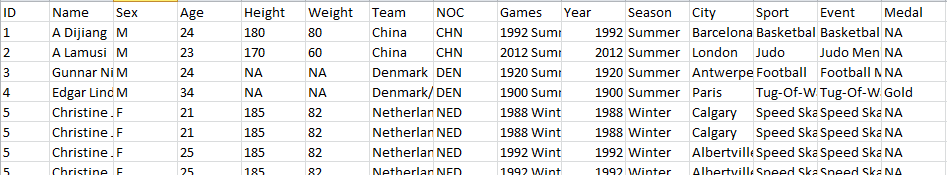
\includegraphics[width=0.95\textwidth, frame]
                        {./images/data/athlete_events.png} 
                    \caption{athlete\_events.csv}                  
                \end{figure}            
            \item NOC regions - A list of the countries and their NOC code. It is important to note some countries changed their code in the data. This is noted in Appendix A. 
                \begin{figure}[H]
                    \centering
                    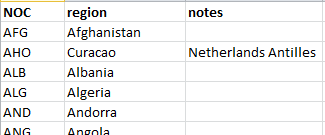
\includegraphics[width=0.4\textwidth, frame]
                    {./images/data/noc_regions.png}   
                    \caption{noc\_regions.csv}                 
            \end{figure}
        \end{enumerate}

    \subsubsection{Country Information}
    The second set of data relates to the information about each country, including their GDP and population. The most trustworthy source for this data publicly available from World Bank national accounts data, and OECD National Accounts data files. The data is available from 1960 to present, and is accessed as separate files. 
        \begin{enumerate}
            \item GDP - The GDP for all countries, represented in current US\$.
                \begin{figure} [H]
                    \centering
                    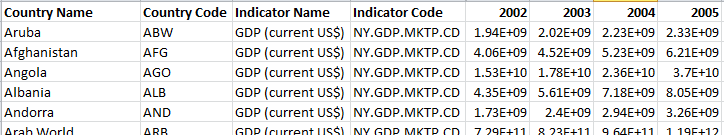
\includegraphics[width=0.95\textwidth, frame]
                        {./images/data/worldbank_gdp.png}
                        \caption{worldbank\_gdp.csv}                    
                \end{figure}
            \item Population - The total population of all countries.
                \begin{figure} [H]
                    \centering
                    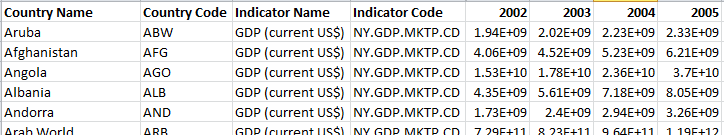
\includegraphics[width=0.95\textwidth, frame]
                        {./images/data/worldbank_gdp.png}      
                        \caption{worldbank\_gdp.csv} 
                \end{figure} 
        \end{enumerate}

    \subsubsection{Host Cities}
    The final set of data is location of each of the games. The 'City' is included as a column in 'athlete\_events.csv', however it is not paired with a country which is needed to compare an athlete's country with where they are competing. This data was not readily available as a data file but the information was found on \url{https://architectureofthegames.net/olympic-host-cities/}. The data was copied into two separate text files as is; summer and winter. Using python the files were read, reformatted and combined to create a csv file. The NOC was also added as an additional column manually using noc\_regions.csv. The file contains the year, city, country, NOC and season of each Olympic games. The code is in Appendix A.1.
        \begin{figure} [H]
            \centering
            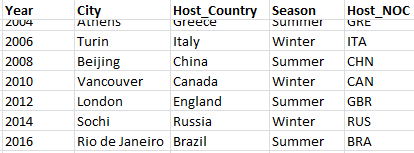
\includegraphics[width=0.5\textwidth, frame]
            {./images/data/host_countries.png}  
            \caption{host\_countries.csv}                  
        \end{figure}  

\subsection{Data Processing}
    \subsubsection{Combined Dataset}
    From all of the above files, a new dataset was created using the python pandas library (and article research) to refine the data selection, remove redundancies, combine related variables and update incorrect data to ensure a cleaner dataset for the visualisations. The code can be found in Appendix A.2. These steps were taken to combine the athlete\_events.csv, host\_countries.csv and noc\_regions.csv:
        \begin{enumerate}
            \item Remove 'Art Competitions' 
            \item Remove 'Name', 'Team' from athlete\_events.csv
                \begin{itemize}
                    \item 'Name' - the identification of the athletes is not important
                    \item 'Team' - sometimes contradicts NOC/Country
                \end{itemize}            
            \item Make NOC codes consistent for countries that have changed.            
            % EUA not in athlete_events
            % ROC already accounted for 
               \begin{itemize}
                    \item Singapore (SIN): Stored as SGP in athlete\_events
                    \item Russia (RUS): URS (1952-1988), EUN (1992), RUS (1994-2018)
                    \item Taiwan (TPE): ROC (1952-1976), TPE(1984-2018)
                    \item China (CHN): ROC (1924-1948), CHN (1980-2018)
                    \item Germany (GER): GER (1896-2018), EUA (1956-1964), FRG \& GDR (1968-1988)
                    \item Czech Republic (CZE): CZE (1994-2018), TCH (1920-1992), BOH (1900-1912)
                    \item Serbia (SRB): SCG (2004-2006), SRB (1912, 2008-2018), YUG (1920-2002)
                \end{itemize}            
            \item Add column COUNTRY by matching ‘NOC’ with the same from noc\_regions.csv
            \item Update host CITY in athlete\_events.csv to match more common names used in host\_cities.csv
                \begin{itemize}
                    \item Athina to Athens
                    \item Roma to Rome 
                    \item Antwerpen to Antwerp
                    \item Moskva to Moscow
                    \item Torino to Turin
                    \item Sankt Moritz to St Moritz
                \end{itemize}                 
            \item Add column HOST NOC by matching ‘NOC’ with same from host\_city.csv
            \item Add column for BMI using the formula Weight (kg) / Height**2 (m) 
               \begin{itemize}
                    \item Height is centimetres in dataset, needs to be converted to metres (Height / 100)
                \end{itemize}
            \item Add column with Boolean value corresponding to whether an athlete is a medal winner     
            \item Add column GDP by matching ‘country’ in gdp.csv
                \begin{itemize}
                    \item File listed with years as columns
                    \item 'melt()' the table to create row entry for each NOC and year
                    \item Convert values to billions (divide by 1,000,000,000)
                \end{itemize}
            \item Add column POPULATION by matching ‘country’ in population.csv  
                \begin{itemize}
                    \item The same procedure as GDP
                    \item Convert the values to millions (divide by 1,000,000)
                \end{itemize}
        \end{enumerate}
    
        \begin{figure} [H]
            \centering
            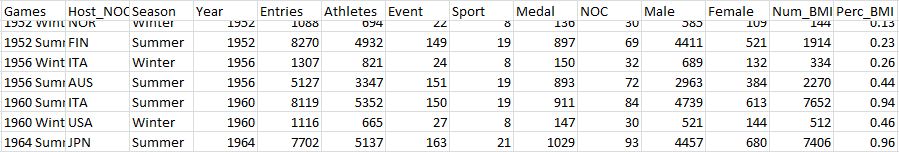
\includegraphics[width=0.95\textwidth, frame]
                {./images/data/games_draft.png}     
            \caption{games\_total\_draft.csv}               
        \end{figure} 

    At this point, the data was looked at more intensely and some preliminary graphs were tested. After reviewing this information, there were a few additional changes to be made. The data at this stage was saved to a separate file. 
        \begin{enumerate}
            \item Remove Years 1896-1952 from athlete\_events.csv
                \begin{itemize}
                    \item Women didn't compete in 1896
                    \item Winter Games didn't commence until 1924
                    \item China and USSR joined in 1952
                    \item Since 1960, the recording of weight and height is more than 90\% 
                    \item The GDP and population is not available until 1960
                \end{itemize}
            \item Remove 'Winter' season, as not only will this overcomplicate the results and comparisons, but also Summer has a lot more data which will skew the outputs.
                \begin{itemize}
                    \item Summer has 2.3 times more countries each year
                    \item Summer has 2.3 times more sports each year
                    \item Summer has 4 times more athletes competing
                    \item summer has 3 times more events
                \end{itemize}
            \item Remove 'Season' and 'Games' columns   
                \begin{itemize}
                    \item Season is no longer relevant since only looking at Summer
                    \item Games was unique identifier between seasons, without season comparison it is just a duplicate of Year and Season
                \end{itemize}             
        \end{enumerate}

    With these changes, a new table was created with just Summer Olympics from 1956 with the above data. The code for this process is in Appendix A.2.      
        \begin{figure} [H]
            \centering
            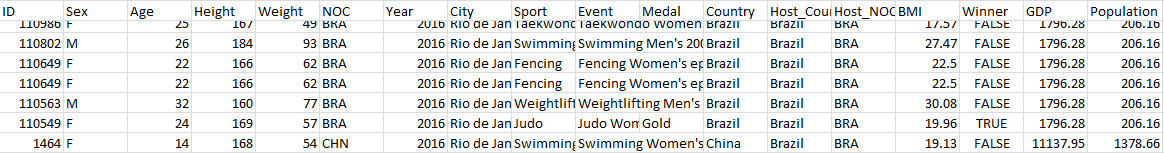
\includegraphics[width=0.95\textwidth, frame]
                {./images/data/all_data.png}      
                \caption{all\_data.csv} 
        \end{figure}

    \subsubsection{Totals}
    To adequately explore the summer dataset there were a number of aggregations that needed to be performed to calculate the total values of certain variables. Using panda data frames new subsets of the data were created to allow repeated access to these aggregations. The code is in Appendix A.3.
        \begin{enumerate} 
            \item \textbf{The Athletes} - This subset was created to refine the information relating to the individual athletes. This dataset is not considered with the type of sports or events the athlete participates in nor the year. 
                \begin{itemize}
                    \item Group the athletes by their ID so there is only one row per athlete, rather than a row for each entry by that athlete
                    \item Count the number of different sports the athlete competes in
                    \item Count the number of entries the athlete has in the summer dataset
                    \item Update the sex labels from 'M' to 'Male' and 'F' to 'Female'
                \end{itemize}
                \begin{figure} [H]
                    \centering
                    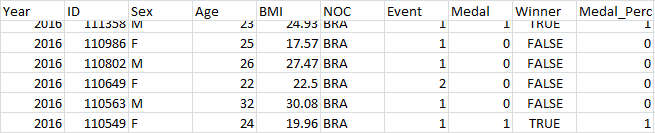
\includegraphics[width=0.95\textwidth, frame]
                        {./images/data/athlete_total.png}      
                        \caption{athlete\_total.csv} 
                \end{figure}

            \item \textbf{The Games} - This table breaks down the data into one entry per Games. It records the year and host country as well as the number of entries, events, sports, athletes (also broken down into Male and Female) and medals (also split into host and visitor amounts and percentages.)
                \begin{itemize}
                    \item Group the entries by the year, so there is only one entry per games
                    \item Keep column with Host Country Code
                    \item Count the number of entries for that year, store as 'Entries'
                    \item Count the number of athletes for that year (one entry per athlete ID) as 'Athletes'
                    \item Count the number of unique events held that year as 'Event'
                    \item Count the number of unique sports hosted that year as 'Sport'
                    \item Count the number of medals awarded that year as 'Medal'
                    \item Add column 'Host\_Medal' to record number of medals awarded to host country
                    \item Add column 'Visitor\_Medal' to records all medals not awarded to host (total - host)
                    \item Count how many male athletes entered as 'Male'
                    \item Count how many female athletes entered as 'Female'
                    \item Calculate the percentage of medals awarded to the host
                    \item Calculate the percentage of medals awarded to all others
                \end{itemize}
                \begin{figure} [H]
                    \centering
                    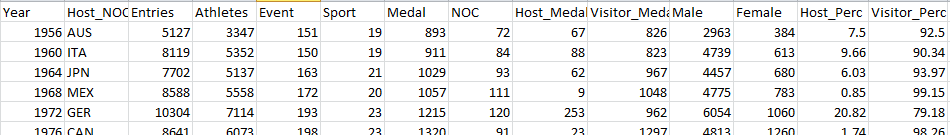
\includegraphics[width=0.95\textwidth, frame]
                        {./images/data/games_total.png}      
                        \caption{games\_total.csv} 
                \end{figure}

            \item \textbf{The Countries} - Finally, this dataset looks at the data from the perspective of the countries participating. There is an entry for each country and each games they compete it. As well as their code and name, this table also includes the GDP and population for the year, whether they were the host that year, as well as the same information as the games, except country specific.
                \begin{itemize}
                    \item Group the entries by the year and country code
                    \item Keep columns for country code, name, GDP, population and host 
                    \item Count the number of entries for that year, store as 'Entries'
                    \item Count the number of athletes for that year (one entry per athlete ID) as 'Athletes'
                    \item Count the number of unique events held that year as 'Event'
                    \item Count the number of unique sports hosted that year as 'Sport'
                    \item Count the number of medals awarded that year as 'Medal'
                    \item Count how many male athletes entered as 'Male'
                    \item Count how many female athletes entered as 'Female'
                    \item Include number of medals and entries for each games
                    \item Calculate the percentage of medals awarded to the country from the total
                    \item Calculate the percentage of entries from the country compared to the total
                    \item Calculate the average number of events per athlete to determine uniqueness
                    \item Add column of Boolean whether country is in top 20 of total medals since 1956
                    \item Add column of Boolean whether country is in top 10 of total medals since 1956
                \end{itemize}
                \begin{figure} [H]
                    \centering
                    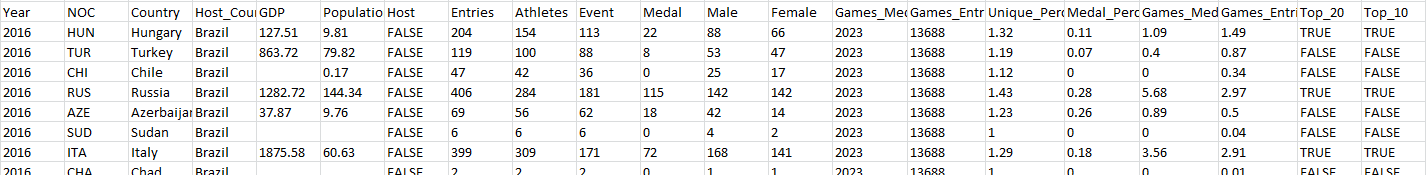
\includegraphics[width=0.95\textwidth, frame]
                        {./images/data/noc_total.png}      
                        \caption{noc\_total.csv} 
                \end{figure}

            \end{enumerate}



\section{Discussion}
The prediction of medal winners will be explored through a number of topics. Due to the difference in data size and added complexity, as explained in the data section, only data from the Summer Olympics since 1956 will be considered. The following questions will be explored and discussed.
            \begin{itemize}
                \item How have the games changed?
                \item What are the characteristics of an Olympic Athlete?
                \item Is there a difference in physicality between athletes and winners?
                \item Which countries are the best at the Olympics and how do they differ?
                \item Does the competition provide equal opportunity to all countries?
            \end{itemize}


    \subsection{The Games}
    There are many factors associated with the Olympic games including the number of entries, athletes (male and female), countries, events, sports and medals. To show how the Olympics has changed over time, in this instance the data set of interest (after 1955) will be compared with the data before 1955. This is the only graph that includes data before 1955. The data used is from the games\_totals.csv. The below histogram provides a sense of the distribution of these factors for all Modern Summer Olympics. A histogram is used to show how many occurrences there are of a single variable and grouping the data into bins (i.e. sets) to give a preliminary idea of the data. Additionally, the data was separated into two subgroups; games before and after 1955.
        \begin{figure} [H]
            \centering
            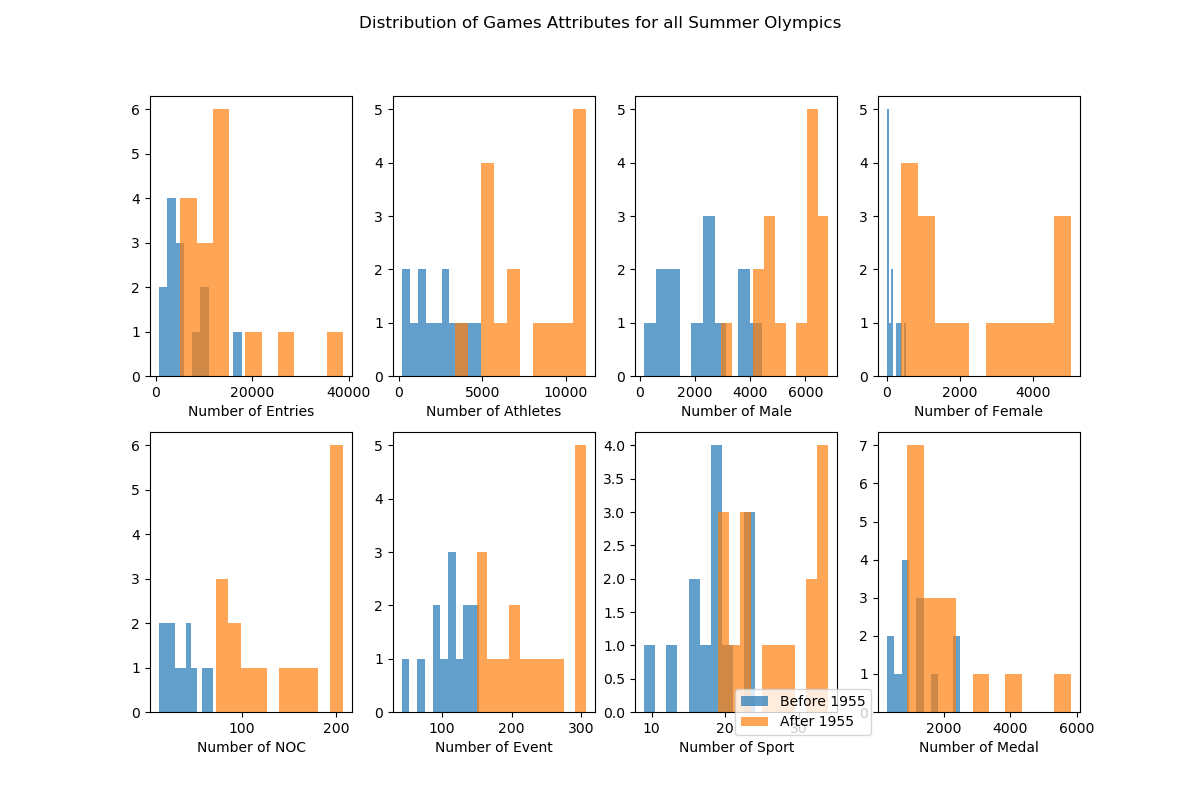
\includegraphics[width=\textwidth, frame]
                {./images/graph/games_histogram.png}      
                \caption{Distribution of variables in Games} 
        \end{figure}
    It is evident that the games have changed since the first 60 years of competition. All of the factors are considerably higher after 1955. Notably the number of women prior to 1955 was never higher than 500 competitors, but after this time, at least half of the games has seen more than 3,000 female competitors. Also, the number of countries competing has more than doubled with 6 of the games in the last 60 years seeing approximately 200 countries competing. From this graph it is evident that the Summer Olympic games have significantly diversified and become more accessible to more athletes around the world.

    \subsection{The Athletes}
    Without the athletes there would be no Olympic Games, so naturally the next topic to explore are the characteristics of the Olympians themselves. Besides their country and their sport of choice, the defining characteristics of an athlete are their Age and BMI. Other interesting factors include how many events they compete in and how many medals on average an athlete wins. All of these graphs use the data of the totals for each unique athlete from athlete\_total.csv.
    
        \subsubsection{Age}
        To explore the change in age of athletes the below boxplot shows the central tendency of athlete's age over the last 60 years of games. Additionally, the data is split by an athlete's sex to show the difference between male and female over time. A boxplot shows the spread of data as a compact alternative to a histogram, which highlights the general nature of the data. It identifies the median and interquartile range (25th to 75th) percentile as the box, as well as low and high adjusters with outliers consistently. Due to the high number of athletes, a boxplot was the ultimate choice to display this data as the median and interquartile range are not impacted by outliers allowing a clear view of the general trends of the athletes. 
        \begin{figure} [H]
            \centering
            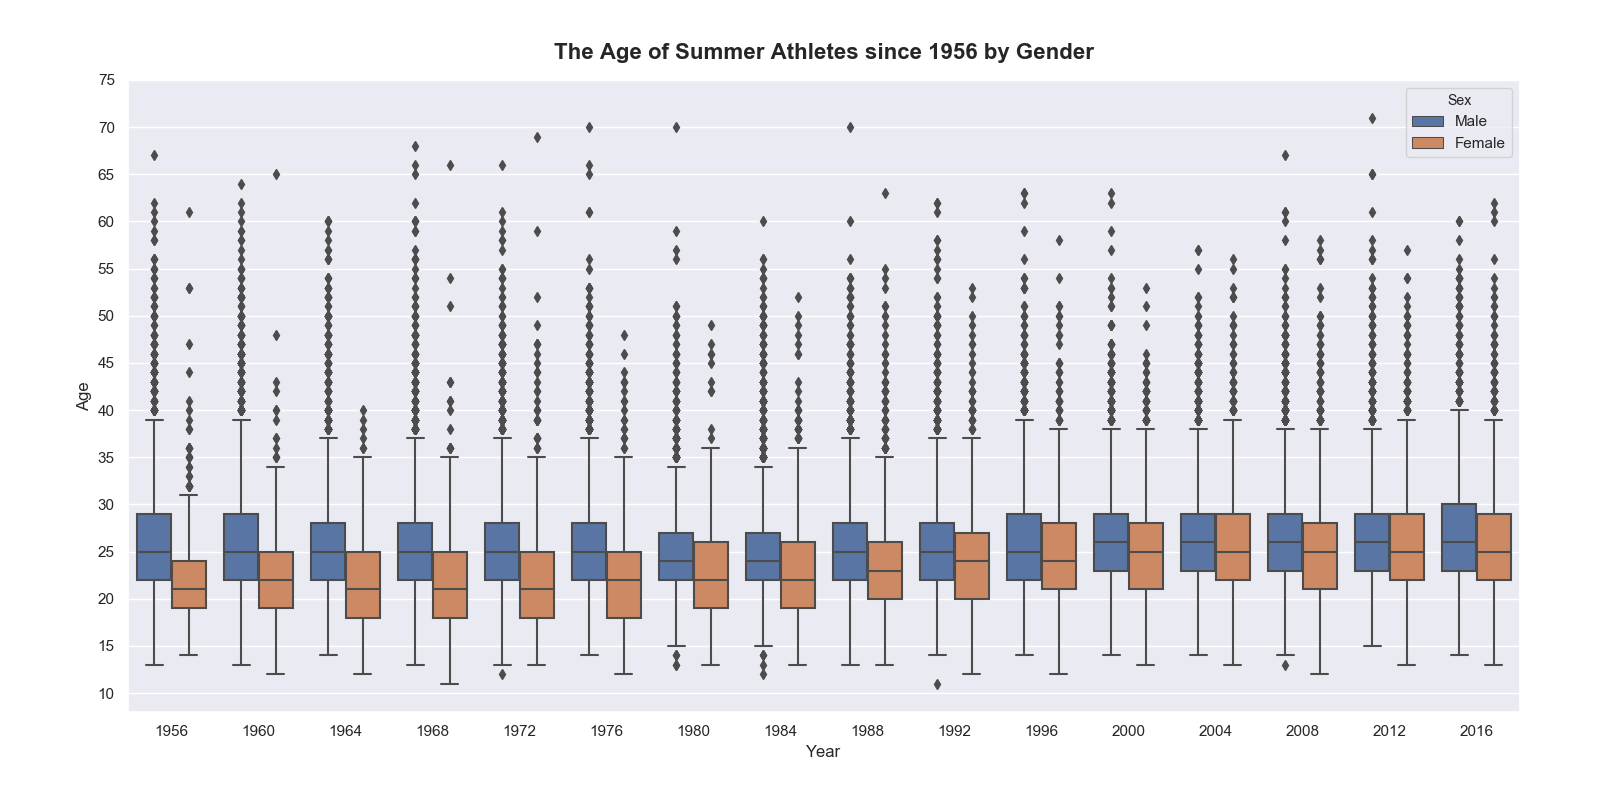
\includegraphics[width=\textwidth, frame]
                {./images/graph/athlete_age_boxplot.png}      
                \caption{Distribution of Age of Athletes by Year} 
        \end{figure}
         
        \textbf{Male:} From this boxplot it is evident that the age of male athletes has remained fairly consistent.  Overall the median age for males has fluctuated between 24 and 26 years old (where it currently stands) and the interquartile range has simply moved up one year.
        \begin{itemize}
            \item Median: 
                \begin{itemize}
                    \item 25 years old: 1956 to 1976, then dropped slightly to,
                    \item 24 years old: 1980 to 1984, before returning to,
                    \item 25 years old: 1988 to 1996, then increasing to 
                    \item 26 years old: 2000 to 2016. same.
                \end{itemize}
            \item Interquartile Range:
                \begin{itemize}
                    \item The 25th percentile value over time has only increased from 22 to 23 years old.
                    \item The 75th percentile has increased from 29 to 30 years old
                \end{itemize}
        \end{itemize}

        \textbf{Female:} From the boxplot, it is clear that female athletes in general are younger than men with lower percentile values. The median age of females has increased by four years from 21 to 25 years old. Also, the interquartile range for females has seen a more dramatic change from 19 and 24, to 22 and 29. Not only has the range shifted up by 3 years but also expanded by 2 years. As the histogram showed that the number of women competing has increased then it can also be assumed that more older woman are becoming eligible to compete as well. 
        \begin{itemize}
            \item Median:
                \begin{itemize}
                    \item 21 years old: 1956, then fluctuating to 
                    \item 22 years old: 1960 to 1984, then increase today
                    \item 23 years old: 1988, then increase again to
                    \item 24 years old: 1992 to 1996, then increase again to 
                    \item 25 years old: 2000 to 2016.
                \end{itemize}
            \item Interquartile range:
                \begin{itemize}
                    \item The 25th percentile decreased from 19 to 18 until 1976, before continuing to increase to 22 in 2004.
                    \item The 75th percentile value has continued to increase from 24 to 29. 
                \end{itemize}
        \end{itemize}
        Another interesting observation is that male athletes always appear to have more outliers in their age, however the number of outliers for women is increasing.

        \subsubsection{BMI}
        The BMI of an athlete is determined by athlete's height and weight. The equation is weight (kg) multiplied by the height (m) squared. To explore another method of viewing the central tendency distribution of a variable the change in athlete's BMI has been shown with a violin plot. Similar to the boxplot, it shows the median, interquartile range and outliers. The main difference is that instead of clear guidelines for the ranges and specific points representing the outliers, the violin plot represents this data with a kernel density estimation to show very general trends. This makes it perfect options for BMI as the interquartile range is small, compared to the extension of the outliers. The graph is also split between gender to see the difference. 
        \begin{figure} [H]
            \centering
            \includegraphics[width=\textwidth, frame]
                {./images/graph/athlete_BMI_violinplot.png}      
                \caption{Distribution of BMI of Athletes by Year} 
        \end{figure}
        From the plot, it is again evident that the values for females are slightly lower. It is also clear that the general trend of BMI within the male and female groups are the roughly the same, with similar sized density shapes. The median and interquartile ranges for both genders has remained almost consistent for the last 60 years. Males range from 22 to 25, with a median of approximately 23.5, whilst females range from 20 to 23 with a median of approximately 21.5. The biggest variation over time has been the number of outliers. It appears in the last 5 games the variation of outlier has increased since 1992 from 50 to 65. This graph suggests that the BMI of most athletes has not changed in the last 60 years, though in some events a higher BMI is advantageous.

        \subsubsection{Events}
        The next aspect of an athlete is the number of events they participate in. By exploring this topic, some insights into how diverse the athlete is can be gained. To plot this data a bar graph was used, due to the very small variation in the behaviour of most athletes and the extremes of the outliers. A bar graph calculates the mean and a confidence interval around this estimate which is displayed with error bars. 
        \begin{figure} [H]
            \centering
            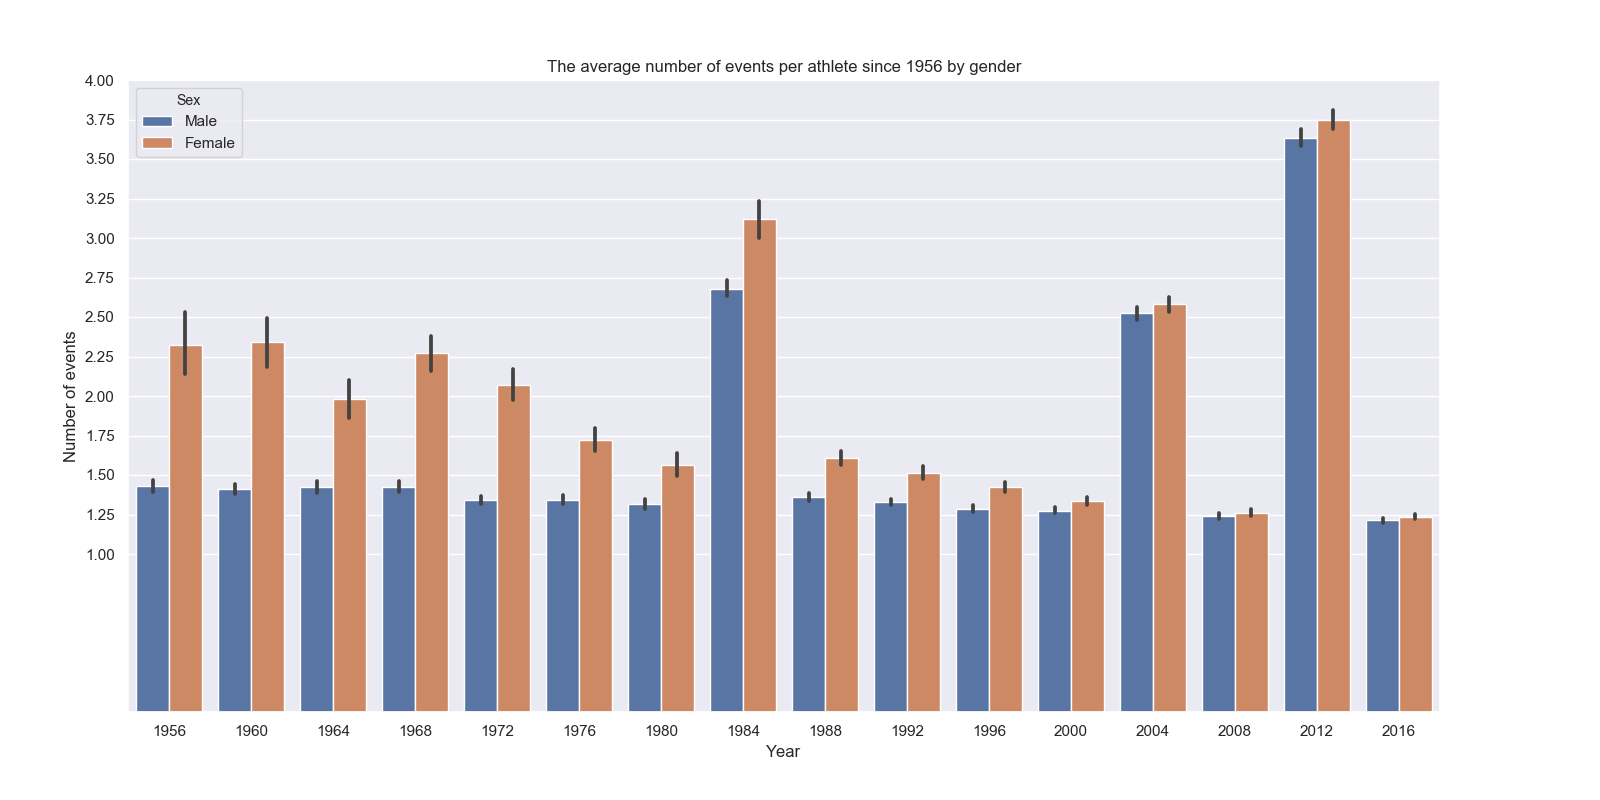
\includegraphics[width=\textwidth, frame]
                {./images/graph/athlete_event_barplot.png}      
                \caption{Distribution of Average Number of Events per Athlete} 
        \end{figure}
        The first observation to note is that the number of events competed in by each athlete increase by almost 1.5 events from the previous year in 1984, 2004 and 2002.  Taking another look at the data and games histogram, it is evident that there are a least 3 games that experience at very large increase in number of entries and medals awarded. 

        Males: The number of events on average of only changed from approximately 1.4 events to 1.25 over the last 60 years, not considering the three outlying years. The error bar has also remained the same and small. 

        Females: From 1956 to 1960, the number of events per female is almost 1 event extra than males. The trend of being higher continues for the rest of the games, although it decreases considerably by 2000. Ignoring the outlying years, the number of events per female has decreased from 2.3 (almost 1.5 events more than males) to be almost the same average as males of 1.25 events per athlete. Also, the error bar decreases greatly to be consistent with males from 1988. These trends could be related to the greatly increased number of female athletes and opportunities for more diversified athletes, as per the histogram.         

        \subsubsection{Medals}
        Another aspect of an athletes participation behaviour at the Olympics, and potentially the most important to them, is the number of medals awarded to each athlete. By exploring this data it may provide insight into whether the medals are being awarded to a variety of athletes, or if the games rely on 'super' athletes winning all of the medals. This data is displayed using a point plot. Similar to the bar plot it computes the mean and a confidence interval with error bars, additionally it joins the points together to help visualise a pattern over time. 

        \begin{figure} [H]
            \centering
            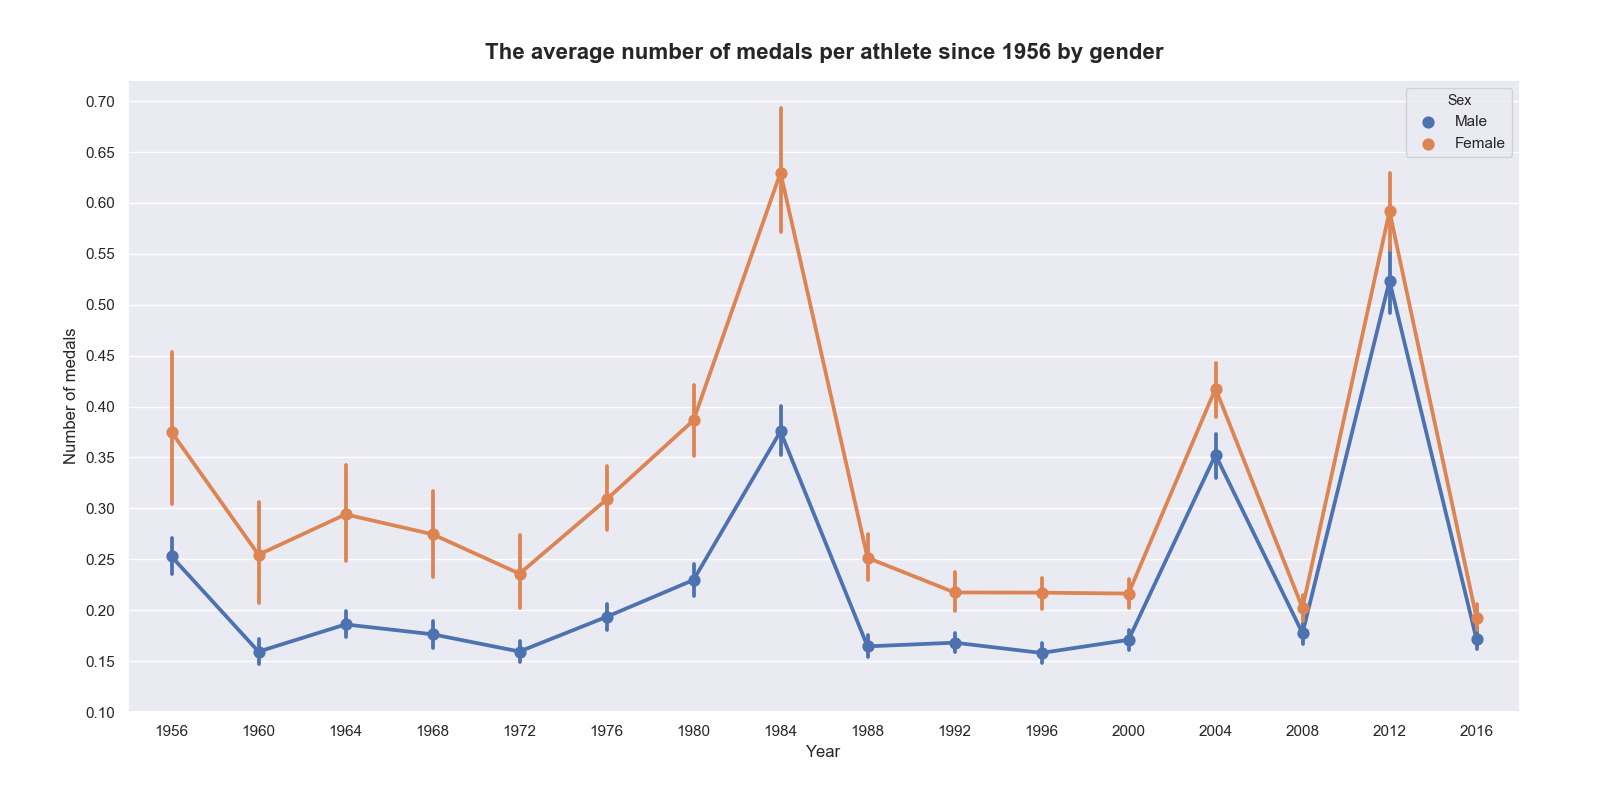
\includegraphics[width=\textwidth, frame]
                {./images/graph/athlete_medal_pointplot.png}      
                \caption{Distribution of Average Number of Medals per Athlete} 
        \end{figure}
        Again this plot shows a spike for athletes in 1984, 2004 and 2008, which is explained previously. Additionally, the higher values in 1956, 1976 and 1980 maybe be explained by boycotts by various nations during these year, decreasing the competition in events and allowing an individual athlete more opportunity to win medals. On average an event will have 8 entries, 3 of which will receive a medal. This means if each entry at the Olympics was filled by a different athlete the average number of medals should be 0.375 for completely equal distribution.          

        Males: Not accounting for the above outlying years, the average number of medals has remained around 0.15 per athlete. Also, the error bars are greater than those seen in the average number of events plot, suggesting more variation from the average. Since the average number of events per male athlete is 1.25 and as mentioned the average number of medals for equal distribution is 0.375, this suggests that more athletes are not winning a medal, whilst a smaller group are dominating the medal count.

        Females: On the graph it is apparent that female athletes on average win more medals, though the gap between male and female as been closing since 1988. The error bars are also much greater than that of male athletes. The average, ignoring outlying years, for number of medals awarded to each athletes has decreased from 0.25 to 0.18. The difference between males and females follows the same pattern as the average number of events, suggesting that the same females are winning the medals across a number of events. 

        \subsubsection{Medal Winners}
        Naturally the next topic to discuss is whether the physical characteristics of athletes who win a medal and athletes who don't differ. Since the average number of medals per athlete is only approximately 0.15 there is a big difference in the amount of data points for medallists and non medal athletes. Therefore, to be able to view the relationship between the two the below are two QQ (Quantile-Quantile) plots for age and BMI respectively. The percentiles of each dataset are calculated and then the corresponding percentiles are plotted against each other. This creates an even number of points for each dataset to be able to compare and view the general trend of their relationship. The standard 45 degree angle is included on the plots to show the linear line if the two datasets had equal percentiles. Additionally the median (50th percentile) and interquartile range (between 25th and 75th percentile) have been included for reference.
        \begin{figure} [H]
            \centering
            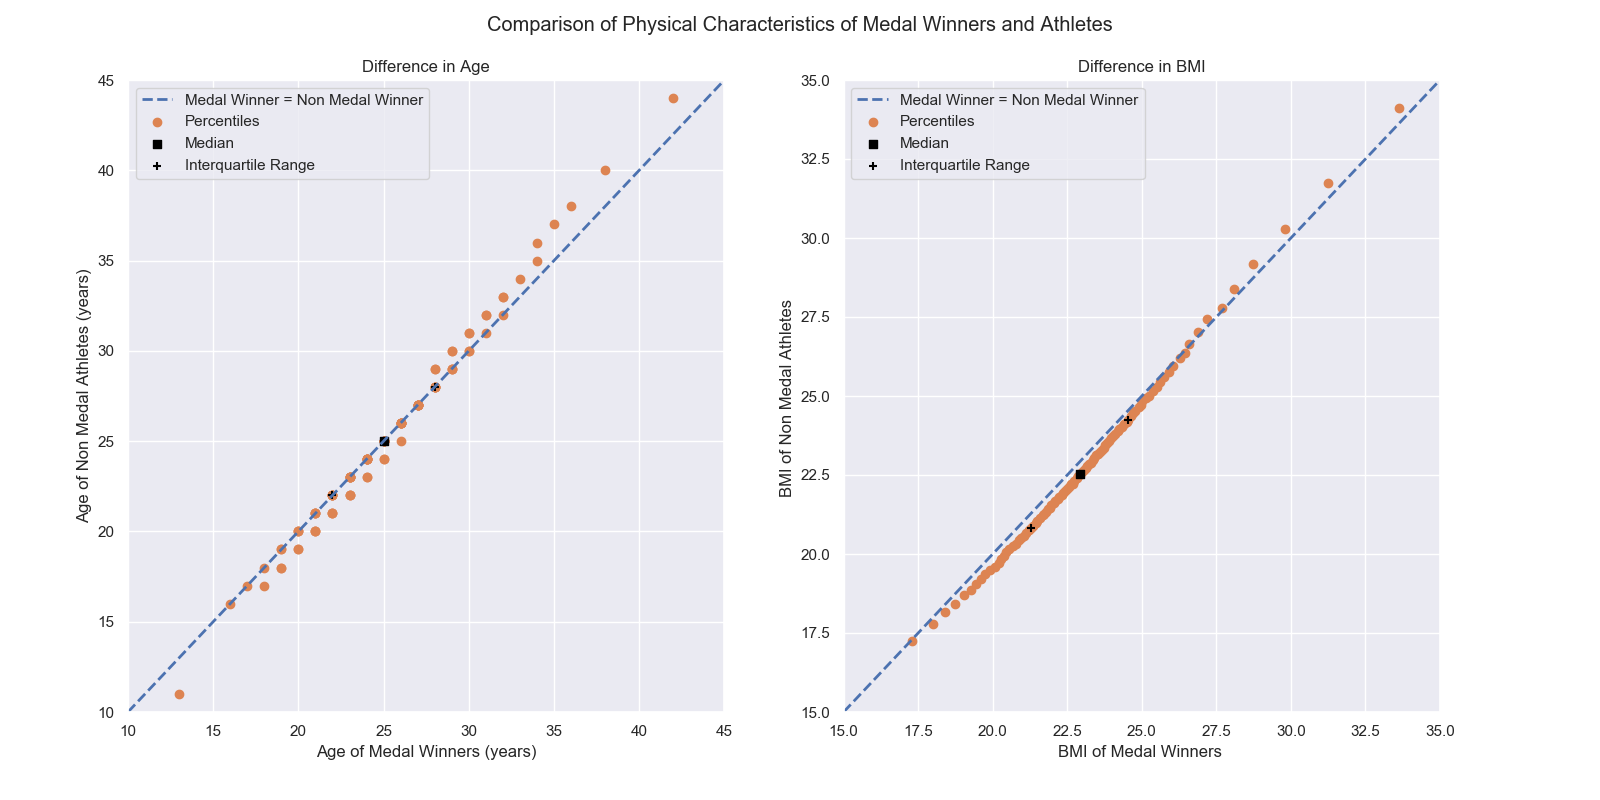
\includegraphics[width=\textwidth, frame]
                {./images/graph/athlete_difference_qqplot.png}      
                \caption{Comparison of Age and BMI for Medal Winners and Non Medal Athletes} 
        \end{figure}
        
        First, looking at the comparison of age on the left. From the age of 18 to 26 years old the percentiles are either equal or slightly toward the medal winners, meaning the corresponding percentile of the medal winners is slightly higher. This reverses from this point until around age 35, meaning the medal winners are slightly younger during this range. Then from the age of 35 the data points of the non-medal percentiles start to pull away more to a difference of about 2 years. Therefore, medal winners have more athletes older than 18 and younger than 35 years old. 

        Now looking at the BMI on the right, the percentile points are obviously more compact with less variation. It appears that almost 90\% of the data points sit between a BMI of 18.5 and 26.5. There is little deviation from the 45 degree angle, though medal winners appear to have a slightly higher BMI than other athletes. Together these graphs show that the percentiles of each dataset are almost identical. This indicates that the age and BMI of an athlete does not determine how competitive they are going to be at their chosen event.

        It is also important to note that since there is much less data on medal winners than non-medal athletes the percentiles may have some larger gaps, especially for the medallists.
    
    \subsection{The Countries}

        \subsubsection{Hosting}
        Over the last 60 years, there have been 16 Summer Olympics hosted by 14 nations, with both United States and Australia hosting twice. The Olympics have been historically very popular with fans around the world travelling or tuning in to watch the action. It is a well known trope that sporting teams do better when they have the home advantage. The below scatterplot explores whether the same can be said about the Summer Olympics. One of the advantages of a scatterplot is being able to compare two variables and view the relationship between them. The average percentage of medals won by each host country during games when they didn't host, are compared against the percentage (average for AUS and USA) won when hosting. Each point represents a year at the Olympic Games. Included on the plot is a 45 degree angle line to show the points at which the two percentages are equal i.e. hosting has no effect on the percentage of medals won. Additionally on the graph is a robust linear regression model to de-weight outliers with a 95\% confidence interval. 

        \begin{figure} [H]
            \centering
            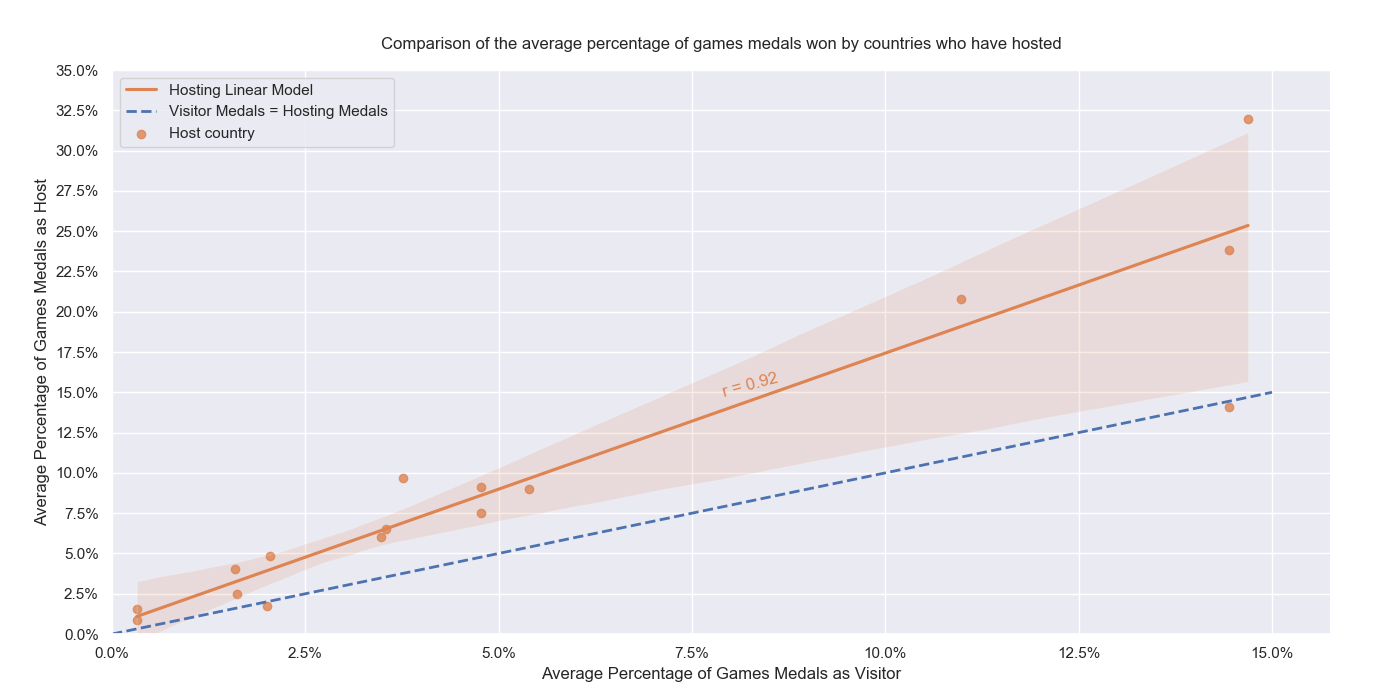
\includegraphics[width=\textwidth, frame]
                {./images/graph/countries_host_lmplot.png}      
                \caption{Comparison of percentage of medals won by host countries} 
        \end{figure}
        From the graph it is very clear that when a country hosts they win a higher percentage of medals compared to when they are a visitor. There are two instances where the percentage is only slightly less, once from a country whom only generally wins around 1.9\% of medals and another country around 14.5\%. Besides these two cases the performance of countries when hosting is far greater than when visiting. The linear regression model seems to be a good fit up until when the confidence interval becomes greater for countries who win more than 5.5\% of medals normally. The outlying values may be explained by boycotts. However, according to the correlation coefficient of 0.92, calculated using Pearson's, the percentage of medals when hosting and visiting are positively correlated and 92\% of the variation in the percentage of hosting can be explained by the linear model fitted.

        \subsubsection{Participation Behaviour}
        Besides hosting, there are a number of other attributes that effect how a country performs at the Olympics. Due to the high number of characteristics and the interest in how each relate to the number of medals awarded to a country, a heatmap is shown. The heatmap shows the Pearson's correlation coefficient for each pair of variables and colour codes it to match. This creates a simple grid to be able to gain quick insights into what variables may have a correlation.

        \begin{figure} [H]
            \centering
            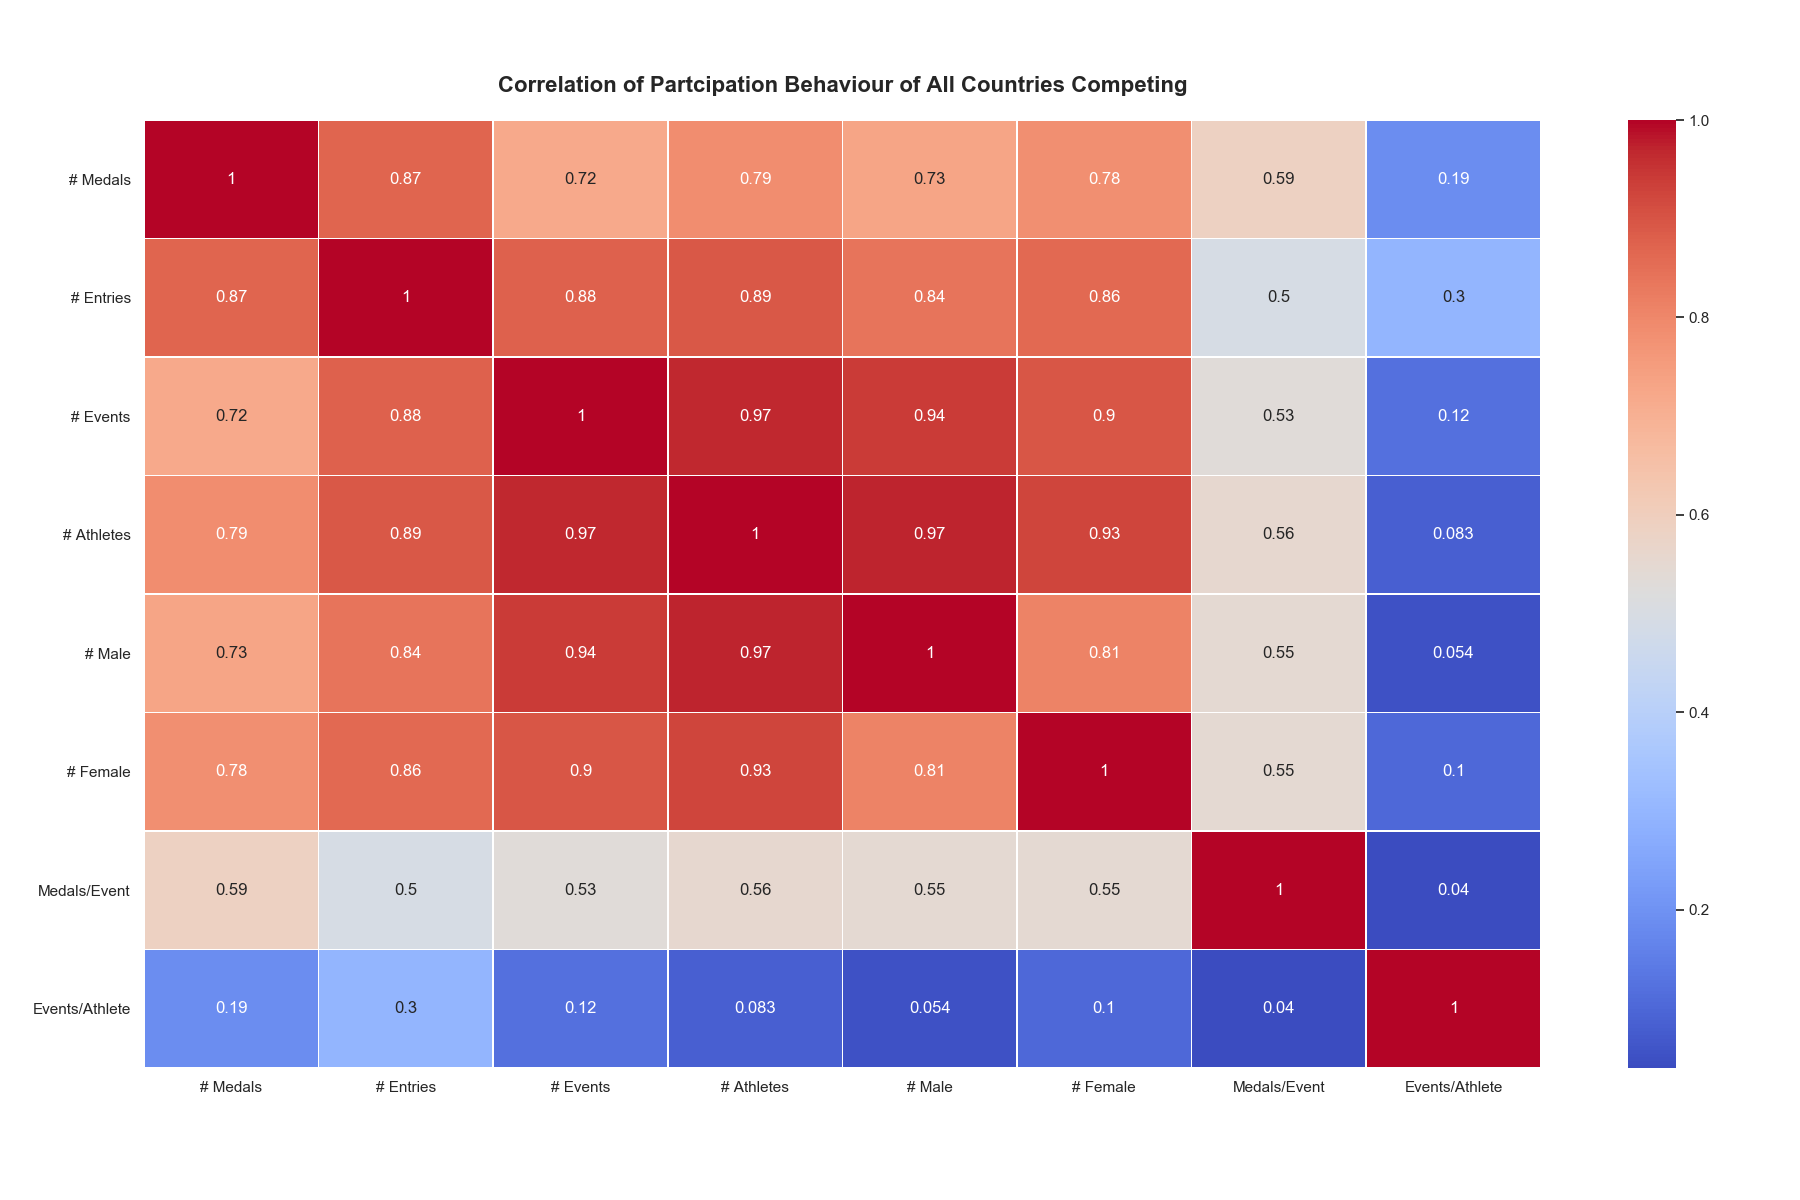
\includegraphics[width=\textwidth, frame]
                {./images/graph/countries_stats_heatmap.png}      
                \caption{Correlation of participation behaviour attributes of countries } 
        \end{figure}

        The strongest correlation to number of medals for a country is the the number of entries (0.87). This intuitively makes sense as the number of entries you have is the same as the opportunities you have to win medals. If there is no difference in general physical characteristics for athletes than simply filling a position increases chances, and the more athletes from the same country in the same event the higher the chance for that country to win at least one of the three medals. The next highest correlation is the number of athletes, with male and female closely following. These correlations suggests that the representation of both male and females impact the number of medals that will be awarded to a country. 
        
        The most surprising observation, in the writers opinion, is that the number of events per athlete seems to have little to no linear correlation to the number of medals (this doesn't change using polynomial fits). Originally the hypothesis was that a country's ability to enter 'super athletes' would correlate well with how many medals would be achieved. But as also supported by the bar graph on the average number of events per athlete which only averaged at 1.25 events, countries too seem to have not much difference in diversification of their athletes.

        \subsubsection{Indicators}
        The next topic to explore is whether barriers exists for countries to fill more entries and hence win more medals. Two of the indicators that may have an impact are the population and GDP of the countries. To demonstrate this multivariate data the below 3D plot shows the relationship of the number of medals, the GDP and population of all countries (with all the available data) for each year from 1960. A 3D graphs allows multiple variables to be displayed to show not only the relationship of variables as pairs but also all together. Shading of points is used to show depth, and colouring based on the number of medals for assisted readability.
        \begin{figure} [H]
            \centering
            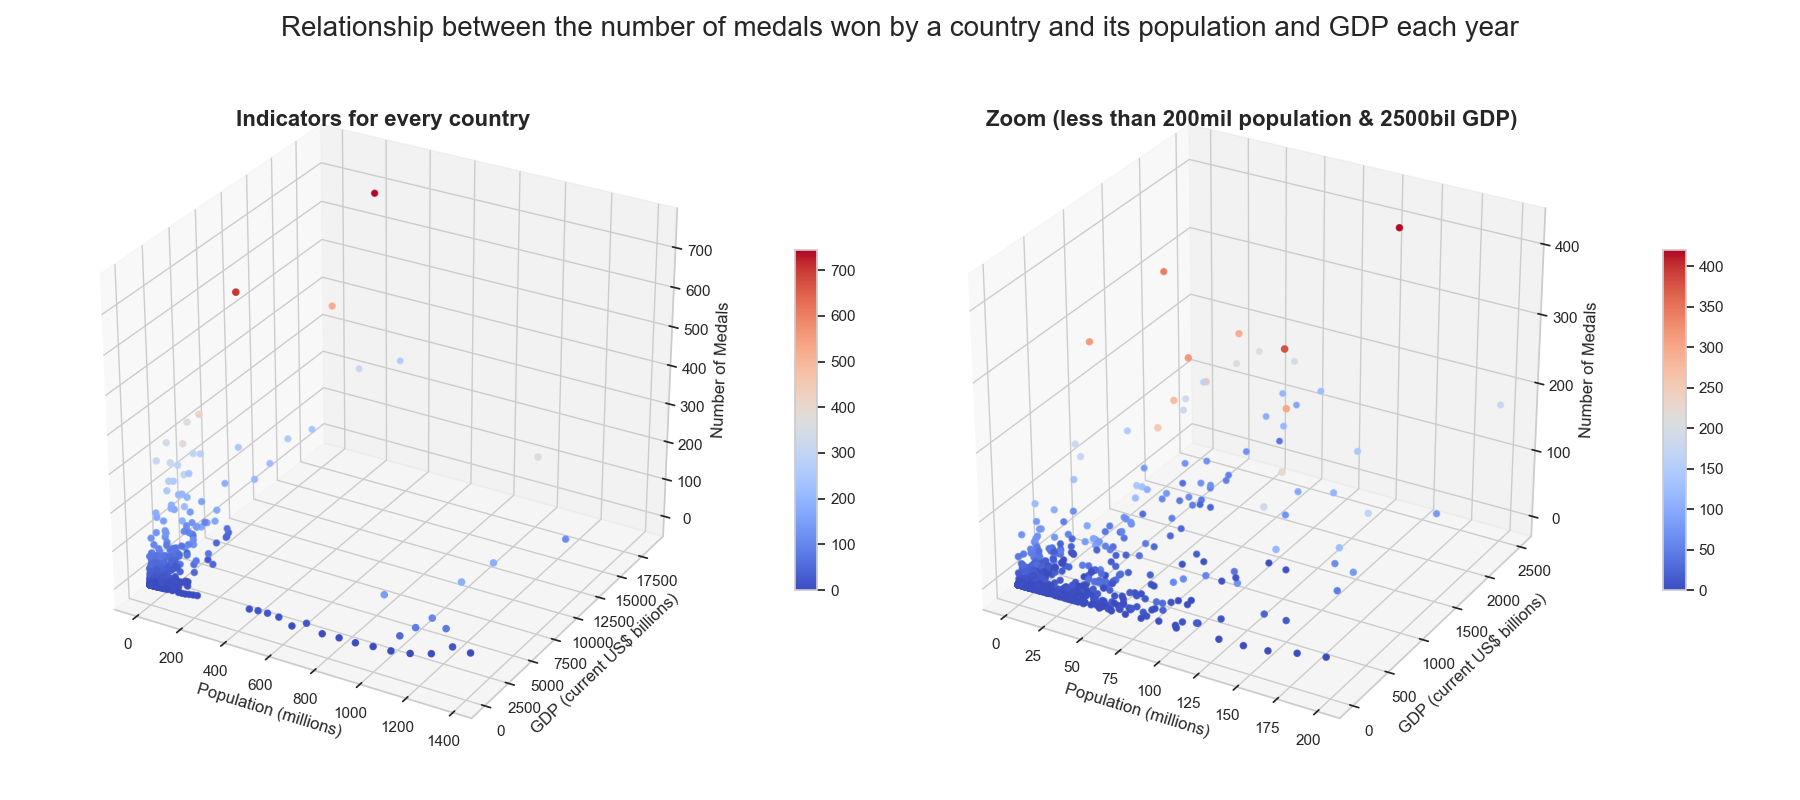
\includegraphics[width=\textwidth, frame]
                {./images/graph/countries_pop_gdp_3d.png}      
                \caption{Population and GDP effect on number of medals awarded to a country} 
        \end{figure}

        Most of the data points lie in a cluster with a population less than 200 million and GDP less than 2500 US\$ billion. Outside of this cluster it appears that the population and GDP have little to do with winning more medals that year. Zooming in on this cluster however shows a general trend of increased number of medals associated with higher GDP and population. Many of the countries are still very clustered and there is not much variation. 

    \subsection{Representation}
    In this section, the aim is to identify whether there is an equal representation of athletes and equal distribution of medals awarded to the countries that participate at the Olympics. The top 10 countries in terms of total number of medals won since 1956 are the USA, Russia, Germany, Australia, China, Great Britain, Italy, Japan, France and Hungary in order. 

        \subsubsection{Entries}
        Due to the strong correlation between the number of entries and the number of medals, the distribution of the number of entries from the top 20 countries with the most number of medals since 1956 will be explored. To account for outliers, the percentage of total entries per game by each of the top 10 countries and the average for each year of the top 11 to 20 countries will be plotted in a swarm plot. A swarm plot groups a variable into categories and then plots the spread of the data with each dot representing a data point (in this case each year). Rather than overlapping points that are the same, the points fan out next to each other. 

        \begin{figure} [H]
            \centering
            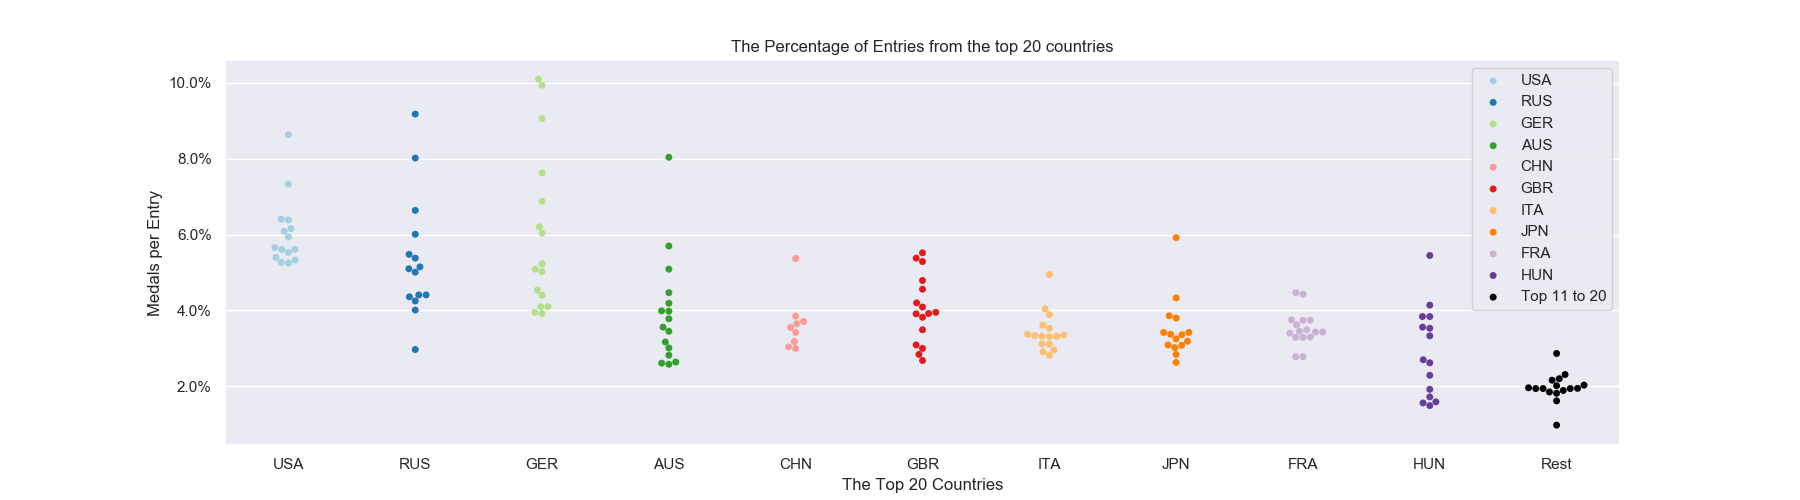
\includegraphics[width=\textwidth, frame]
                {./images/graph/countries_entryperc_swarm.png}      
                \caption{Distribution of entries from countries} 
        \end{figure}

        This graph shows that except for Hungary the percentage of entries from each of the top 10 countries each year is always higher than the average of the top 11 to 20 nations. Besides boycott years, the USA always accounts for at least 5\% of entries, Germany at least 4\% and the remaining except for Hungary account for at least 3\% each. This means that just looking at their minimum contributions, the top 10 nations always account for at least 35\% of the entries at the Olympics. On average the next 10 nations range from 1 to 3\% of the entries. Adding and average of 2\% from these nations, results in the top 20 nations filling at least 55\% of the positions at the Olympics. The 2016 Summer Olympics saw 207 nations competing and 13,688 entries. Therefore, whilst 20 nations enter approximately 7,500 of the available positions, the remaining 187 nations enter only 6,100 positions.


        \subsubsection{Medal Distribution}
        It is clear that the top 10 countries have much higher percentage of entries than other countries. The below stacked bar chart shows how much of the total medals are awarded to the top 10 countries. As mentioned previously a bar chart is in a easy way to represent the count of a variable. In this case, to effectively represent the distribution of 11 groups, a stacked chart clearly shows the distribution and changes of each country.

        \begin{figure} [H]
            \centering
            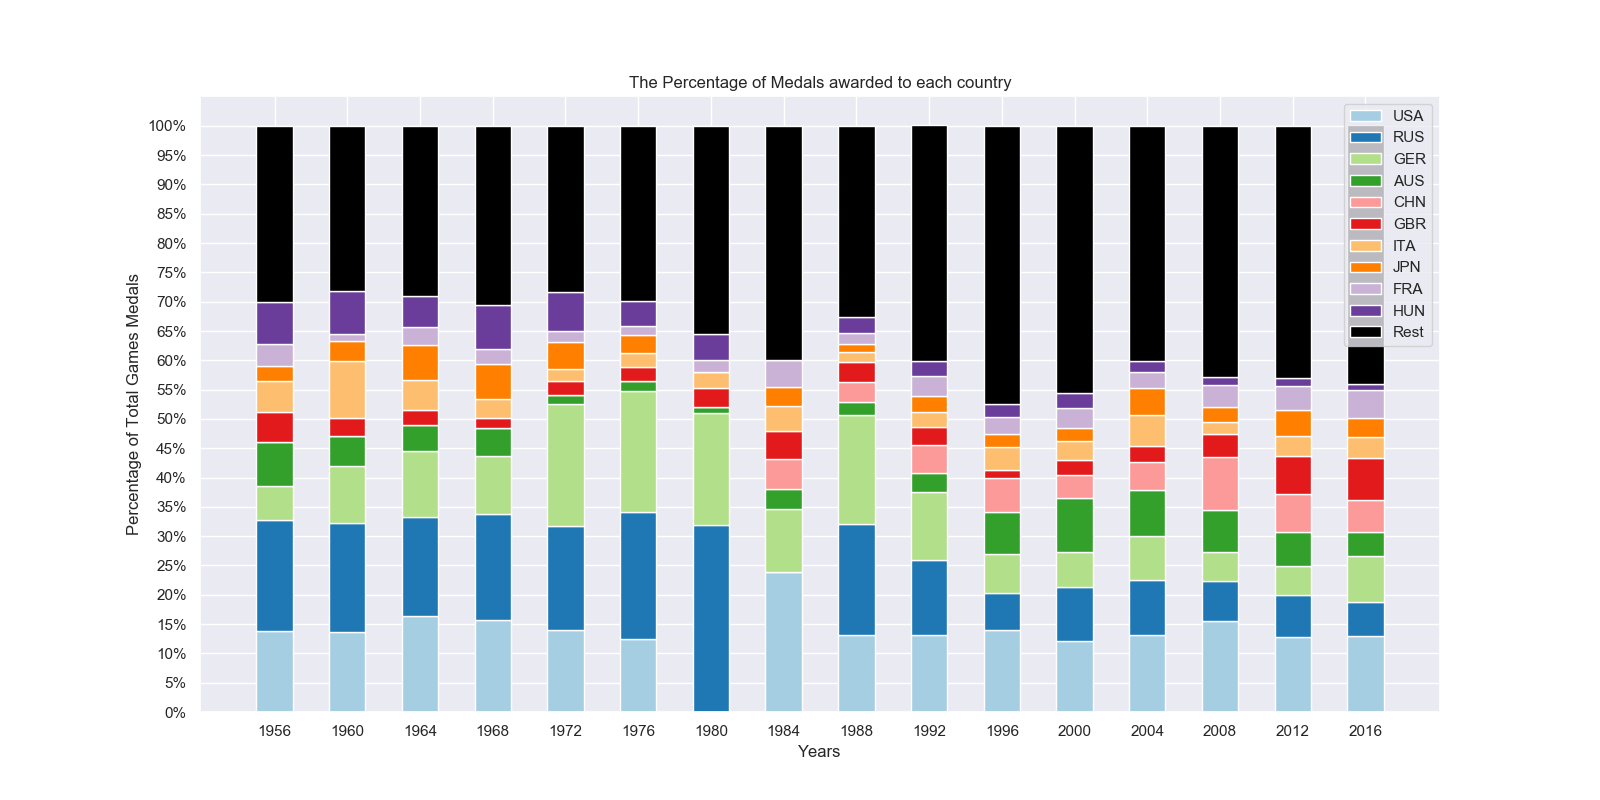
\includegraphics[width=\textwidth, frame]
                {./images/graph/countries_medals_stacked.png}      
                \caption{Breakdown of percentage of medals awarded to each country} 
        \end{figure}

        Rather than representing this chart with total number of medals, a more interesting comparison is to show the percentage of total medals awarded to each country over the years. Using the percentage eliminates outlying years and provides a more consistent representation of the performance of countries. From the chart it is evident that the top 10 countries have consistently dominated the Olympic games, though the domination is easing. The top 10 countries account for at most 70\% in 1956 and at least 52.5\% in 1996 of the total medals awarded. All other nations only account for the remaining percentage of medals. 

        Individually, there are some interesting observations in the top 10 countries. Reminder that during 1980 Games, Russia hosted and there were boycotts from various nations including USA, China and Japan (some athletes from Australia, Great Britain and France), as well as a returned boycott in 1984 where USA hosted and Russia boycotted. China also boycotted the 1956 and 1964 games. The absence on the graph from these countries during these year, prompted the further inspection into these years where this knowledge of boycotts was gained.
        \begin{itemize}
            \item The percentage of medals awarded to Russia has dropped from over 15\% to just around 5\% (ignoring 1980). Interestingly, during 1980 Russia simply accounted for the USA percentage, with little difference to the other top 10 values.
            \item The USA have consistently received at least 12.5\% of the Olympics medals each game.
            \item China is seen entering with more considerable dominance from 1980 increasing to receive 7.5\% of medals (during their year of hosting).
            \item Great Britain, Japan and Italy have fluctuated without much pattern.
            \item Hungary has continued to decrease from around 6\% to less than 1\%.
            \item Germany has seen some drastic changes in their percentage of medals, ranging from 5\% to 20\% and back again. 
        \end{itemize}          


        \subsubsection{Events}
        The previous heatmap used Pearson's correlation process to determine whether a linear relationship existed amongst the variables. Therefore the possibility of non-linear relationships is yet to be explored. The most interesting relationship using non-linear fits was the number of medals and the number of events. The below graph shows a scatter plot of the top 20 countries with the most medals (the top 10 split individually) and their relationship between the number of medals won each year and the number of different events their athletes competed in. A polynomial fit for all countries can be seen on the graph with a confidence interval of 95\% and to the right are the residuals of this fit.  

        \begin{figure} [H]
            \centering
            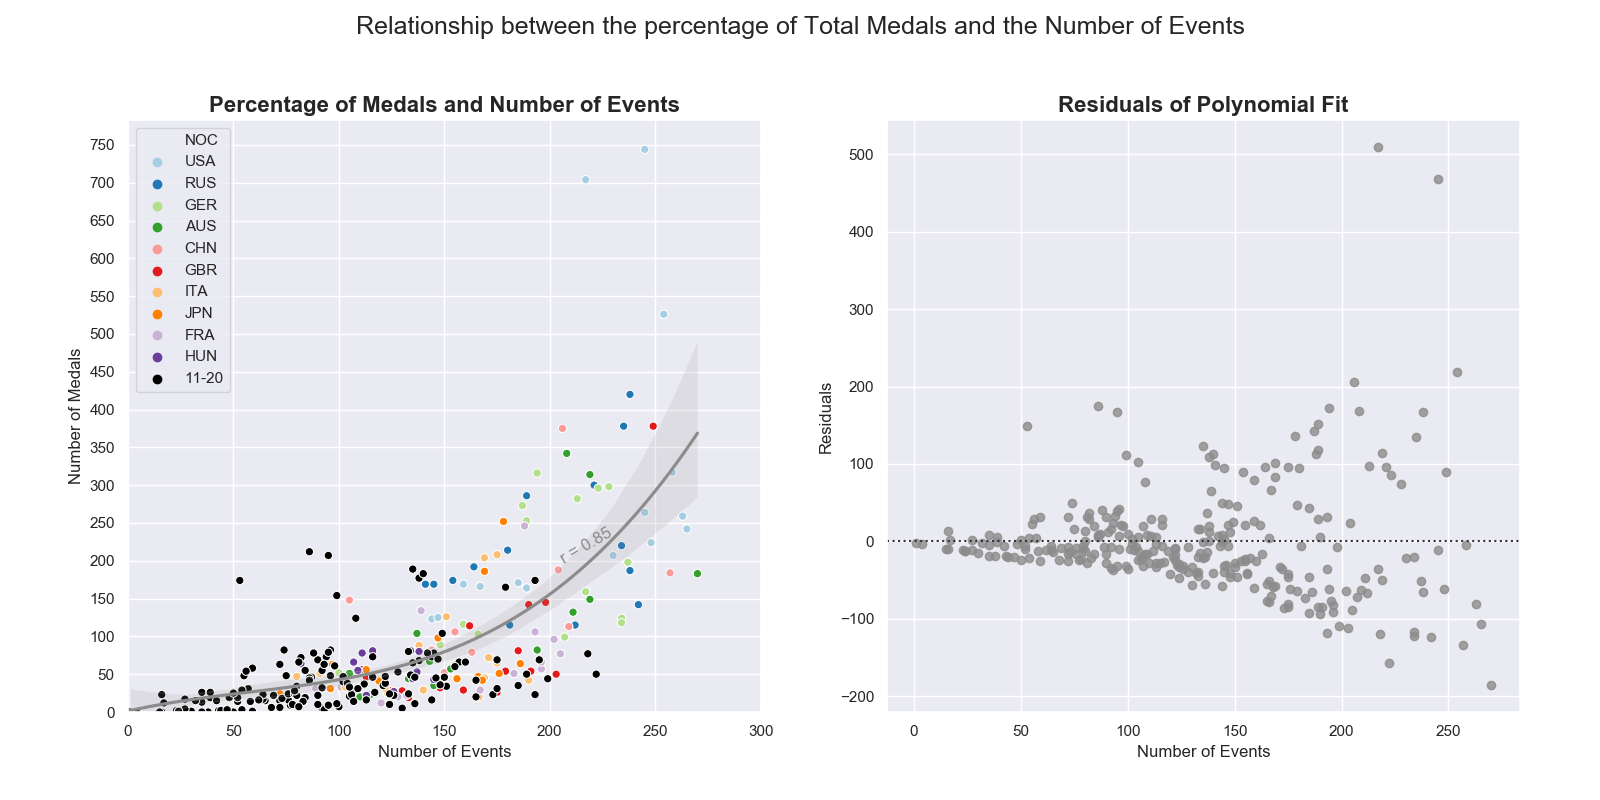
\includegraphics[width=\textwidth, frame]
                {./images/graph/countries_medals_resid.png}      
                \caption{Polynomial Fit and Residuals of Number of Medals and Events} 
        \end{figure}
        For this relationship on the heatmap, the Pearson's correlation coefficient was 0.72, whilst using Spearman's the calculation was 0.79, suggesting a non-linear relationship may be stronger (). Using polynomial fits, and least squares calculations, when the order is increased to 2 (quadratic) the coefficient increases to 0.8. So now instead of 72\% of the data explained, 80\% of the data is explained. However, a quadratic fit for this data causes issues as the fit on the graph showed that if you enter 0 events you can have almost 50 medals which is impossible. Moving up one more order to 3, the least squares coefficient is now 0.85 which not only means these variables are more positively correlated with this fit but also provides a much better and more logical visual fit. Going up another order makes no difference again and so the best fit, without getting any further into complicated algorithms, is a cubic fit. 

        Looking at the residual on the right this pattern is much more scattered that that of the linear plot. However, besides clusters of uniformed scatter, there appears to be unequal scatter overall or heteroscedasticity which may be due to the extremes between the top 10 countries and the rest of the nations (Frost, 2019). 
        
    \section{Conclusion}  
    In conclusion, it is not clear what makes an athlete great or a country 'the best'. Though what is clear from this report is that the opportunity to win a medal at the Olympics has never been better. The games have more sports, events, athletes and countries than ever. There appears to be no difference in the physical characteristics of winners and non-medal athletes. The range for females has increased immensely to be almost on par with males all round. The number of medals a country wins is positively correlated with the number of entries, and diversification of athletes seems to be key. GDP and population of home countries do not appear to be a barrier to most nations winning medals, and whilst there are 10 countries who have won up to 70\% of the medals historically this dominance is decreasing. While no strict conclusions can be made about the equal distribution of the Olympics or whether it is 'fair' the visualisations provide a unique and powerful insight into the last 60 years of the Summer Olympics. 

    \pagebreak
    \section{Reflection}
    Overall, I feel I learnt and implemented a wide range of visualisations that were each fitted for their intended purpose. I analysed univariate, bivariate and multivariate data in different ways to demonstrate my understanding of the multiple ways in which data can be displayed. I learnt and displayed the importance of design choices (such as colour) and accurate labelling.

        \subsection{Design Choices}
        For all of the graphs there was considerable time spent on the design to ensure easy viewing as well as being appealing to the eye. I feel I demonstrated the knowledge I have gained from lectures and research about the importance that style has on a user's ability to interpret a graph accurately.
            \begin{itemize}
                \item The same colours used throughout for consistency and flow.
                \item A grid is displayed on all graphs to assist with reading the values on the graphs as the data is numeric and the specific values are important for analysis.
                \item A grey background is used so that while the grid, is very useful to help read the values, does not take away from the actual points on the graph. Often there are many data points and having a white background with the grid made the grid take away the attention of the points.
                \item A qualitative palette is used for pair comparisons (i.e. male vs. female). The muted version of the default color palette was chosen as it has higher luminance and middle saturation to contrast well with the grey background (seaborn, 2020). This keeps the colours bright but not overpowering. The colours chosen were orange and blue as these contrast well with each other as well as being colour-blind friendly (tableau, 2020)
                \item Categorical colour scheme used for the top 10 countries to assist with representing their order and pairing position 1 with 2, and 3 with 4, etc.
                \item For the heatmap and 3D plot where the difference in extremes of values are displayed a diverging palette is used. I chose 'coolwarm' palette ranging between blue and red to show this range, as well as not stray from the orange and blue used throughout the rest of the report and compliment the background.
                \item Titles on all graphs as well as an additional title for the whole figure if there is more than one plot in the figure.
                \item Legends and axis labels on every graph.
                \item Add units on all axis where needed, including percentage symbols and years in brackets.
                \item Add additional ticks to axis for more accurate reading.
                \item Add frame around each graph to contain it and help it stand out amongst the text of the report.
            \end{itemize}


        \subsubsection{Data Concentration}
        Originally when proposing this project, I wanted to look at both the Summer and Winter Olympics for all modern Olympic years to compare if there was much difference between the two games. The first thing I did was make some preliminary graphs of the univariate data of the athletes; their age, BMI, number of events and number of medals. I was overwhelmed with the number of graphs that it seemed I needed to present the information. Graph with hues to show the difference of a variable depending on season, sex and whether they were a medal winner. But then what about the difference between gender for the season separately, that's another graph each again. 
        
        Also the difference in the amount of data between the seasons was found to be very large, so was comparing the two actually fair? The Summer Olympics saw at least 4 times more athletes each year and this means thousands of more data points used to calculate medians, means and percentiles. It became obvious that the data was skewed. Additionally, when it came to plotting over time, since the Winter Olympics used to be the same year and then switched to alternate years, the graph was squished with an overload of data on the left to then stretching out to the right. This overcrowded the graph and left no room to be able to compare any additional variables. 

        Secondly, when it came to plotting over time, it became apparent that over 100 years of Games was too much to plot at one time. When deciding what year to instead condense the data to I looked at a few factors and decided to take the dataset from 1956 to show the games over a period of 60 years (16 Olympiads).
            \begin{itemize}
                \item 1924: Winter games commence
                \item 1928: Women now compete in more than 2 sports
                \item 1932: Low attendance due to Great Depression
                \item 1940 \& 1944: Cancelled due to WW2
                \item 1952: USSR/Russia starts competing
                \item 1956: Weight and height is recorded for more than 40\% (over 90\% the next year)
                \item 1960: GDP and Population data is available from worldbank
                \item 1984: Mainland China joins the Olympics
            \end{itemize}
        A comparison, despite style, of the readability and knowledge gained from the condensed graphs to what I started with, I think, shows my development in the understanding of sometimes less is more. It is better for users to be able to understand the graph then overload it with all of the information.  

        \subsubsection{Limitations}
        My number one limitation for this project was time. Whilst I spent a lot of time tweaking and rethinking the graphs there is always so much more to do. Some other graphs I would have liked to look into were:
            \begin{itemize}
                \item All of the same graphs for Winter to see the distribution.
                \item Whether an athlete winning one medal increases their likelihood to win more.
                \item Other factors that assist with determining what makes the top 10 countries stand out i.e. spending on sports, average income, contributions by government etc.
                \item Geographical map with animation showing countries being added each year.
            \end{itemize}
        Another limitation I ran into with python plotting was the lack of functionality for logarithmic and exponential graphs. There were some workarounds but they were cumbersome and didn't really produce the results I was looking for and so weren't included. 



        \subsubsection{Key Takeaways}

        \begin{enumerate}
            \item Don't always trust the data - When looking at the relationship between the number of medals per athlete for a country, and the number of medals they win, I noticed three very distinct groupings. I checked multiple times I was selecting the correct data and hadn't made any coding errors but there they still were. I wondered if maybe there were just three distinct groups of behaviour from countries on how good they were at winning medals. However, on closer inspection I came to notice that in fact there were three years of Olympics where there were a lot more events and medals being offered (partially due to new team sports being introduced like golf) which was skewing the data incorrectly.
            \item Reminding myself that correlation does NOT imply causation - Often I found myself trapped in the thinking, 'Well having more athletes means more medals right?' When actually all I was looking at was that the number of athletes positively correlated with the number medals.
            \item Hypotheses don't always come true - There were many times when I thought for sure I knew what the answer would be, 'There must be a difference between medal winners and other athletes', 'A graph with GDP and Population will show that only the rich countries get to compete!' But, data analysis doesn't always work out that way and I learnt the hard way. Graphs that I thought be easy and super clear ended up being confusing with little insight.
        \end{enumerate}




    
        










    \begin{itemize}
        \item The distribution of the number of events and medals [Histogram (\#events, \#medal)]
        


        
        \item The change in age for medal and non-medal winners [Turkey box (year v. age)]
        \item The BMI of medal and non-medal winners [q-q plot (medal v. non-medal BMI)]
        \item The proportion of medal winners to number athletes [scatter (\#athletes v. \#medals)]
        \item The proportion of men and women competing [scatter (\#females v. \#males)]
        \item The difference in \% of medals when competing at host [scatter (\% hosting v. visiting)]
        \item The effect of population and GDP on number of medals [multi \- pop, GDP, \#medals]
    \end{itemize}




% Appendix
\pagebreak
\appendix
\addappheadtotoc
\appendixpage
\section{Important notes about the data}
    \begin{enumerate}
        \item athlete\_events.csv - Possible factors that may affect results of each Olympics
            \begin{itemize}
                \item 1924: Winter games commence
                \item 1928: Women now compete in more than 2 sports
                \item 1932: Low attendance due to Great Depression
                \item 1940 \& 1944: Cancelled due to WW2
                \item 1948: Art sports (architecture, literature, music, painting, sculpture) removed
                \item 1952: USSR/Russia starts competing, Republic of China (ROC) discontinued
                \item 1956: Boycotts by 8 nations, including China
                \item 1960: Height and Weight measured consistently from now
                \item 1976: Boycotts by 25 nations (mostly from Africa)
                \item 1980: Boycotts by 66 nations, including US
                \item 2000: Summer Olympics capped at 28 sports, 300 events, 10,000 athletes                
            \end{itemize}

        \item noc\_regions.csv - The following countries are recorded under multiple codes:
            
        \begin{itemize}
                \item Australia: AUS, ANZ (New Zealand, 1908\-1912)
                \item Russia: URS (1952\-1988), EUN (1992), RUS (1994\-2018)
                \item China: ROC (1924\-1948), CHN (1952\-2018), HKG (Hong Kong, 1952\-2018)
                \item Germany: GER (1896\-2018), EUA (1956\-1964), FRG \& GDR (1968\-1988)
                \item Czech Republic: CZE (1994\-2018), TCH (1920\-1992), BOH (1900\-1912)
                \item Serbia: SCG (2004\-2006), SRB (1912, 2008\-2018), YUG (1920\-2002)                    
            \end{itemize}  

    \end{enumerate}





\pagebreak
\appendix
\appendixpage
\addappheadtotoc
\section{About the data}

    \subsection{Host Cities}
    \lstinputlisting[language=python]{code/host_countries.py}

    \pagebreak
    \subsection{Combined Data}
    \lstinputlisting[language=python]{code/all_data.py}

    \pagebreak
    \subsection{Totals}
    \lstinputlisting[language=python]{code/totals.py}


\pagebreak
\section{Discussion}
    \subsection{The Games}
    \lstinputlisting[language=python]{code/games.py}

    \pagebreak
    \subsection{The Athletes}
    \lstinputlisting[language=python]{code/athletes.py}

    \pagebreak
    \subsection{The Countries}
    \lstinputlisting[language=python]{code/countries.py}

    \pagebreak
    \subsection{Representation}
    \lstinputlisting[language=python]{code/representation.py}









\end{document}